% -*- root: ../../main.tex -*-
\section{Interazioni}
\label{sec:interactions_design}

\subsubsection{Interazione tra Engine, ECS e controller}
Come spiegato nel \ref{sec:ecs_design}, i vari gestori di componenti che compongono l'ECS sono coordinati tra di loro tramite un coordinator. Esso fa da punto di contatto con l'engine vero e proprio esponendo il metodo \emph{updateAllSystems}, che corrisponde a un tick del gioco. Esso viene incapsulato nel metodo \emph{update} esposto dall' interfaccia \textbf{UpdateableEngine}, implementata dal \emph{GameEngine}. In questo modo è possibile per il \emph{GameLoop} interagire con l'engine.
Quando il gioco è fatto eseguire in modalità singleplayer il controller si occupa di creare l'engine e al join di una partita multiplayer esso verrà deallocato e verrà creato l'attore client.
\begin{figure}[H]
	\centering
	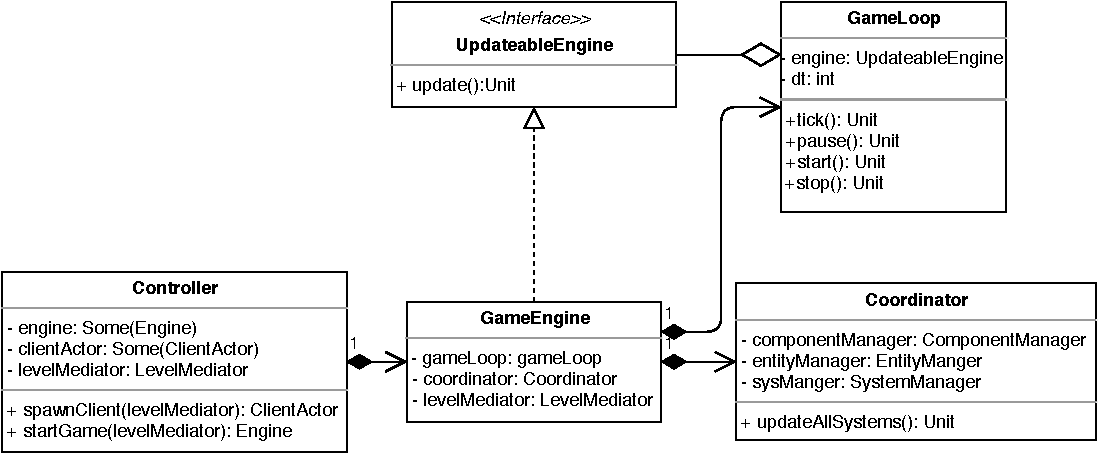
\includegraphics[width=\columnwidth]{drawio/ECS-engine-controller/ecs-engine-controller.pdf}
	\caption{Diagramma raffigurante ecs, engine e controller e le loro interazioni.}
	\label{fig:ecsenginecontroller}
\end{figure}